%%%%%%%%%%%%%%%%%%%%%%%%%%%%%%%%%%%%%%%%%%%%%%%%%%%%%%%%%%%%%%%
%%  Versão final do IEEExplore
%%%%%%%%%%%%%%%%%%%%%%%%%%%%%%%%%%%%%%%%%%%%%%%%%%%%%%%%%%%%%%%

\documentclass[10pt, conference, compsocconf]{IEEEtran}
% \documentclass[a4paper]{sbgames}

\usepackage{times}
\usepackage{graphicx}
\usepackage{amsmath,amssymb,amsthm,siunitx}
\usepackage[brazil,american]{babel}
\usepackage[utf8]{inputenc}
\usepackage{url}

%% use this for zero \parindent and non-zero \parskip, intelligently.
\usepackage{parskip}

%% the 'caption' package provides a nicer-looking replacement
%\usepackage[labelfont=bf,textfont=it]{caption}

\usepackage{url}

\begin{document}

%% Paper title.
\title{The Adventures of Lolo}


\author{\IEEEauthorblockN{Aquila Macedo Costa, Eduardo Ferreira Marques Cavalcante, and Matheus Cardoso de Souza}
\IEEEauthorblockA{Dept. of Computer Science\\
University of Brasilia\\ Brasilia, Brazil\\
Email: {costa.aquila@aluno.unb.br, marques.eduardo@aluno.unb.br, matheus-cardoso.mc@aluno.unb.br}}
}

 % \author{ Autor1
 %         \hspace{28pt} Autor2 \\
 %         \vspace{0pt} \\
 %         {University of Brasília, Dept. of Computer Science, Brazil} }

 % \contactinfo{autor1@gmail.com \\ autor2@hotmail.br }



%\teaser{
%  \includegraphics[width=\linewidth]{sample.pdf}
%  (a)\hspace{150pt} (b) \hspace{150pt}   (c)
%  \caption{(a) Guitar Hero III screen; (b) DE2-35 Kit on top of PlayStation 2; (c) Grybot}
%  \label{fig:01}
%}


% make the title area
\maketitle

% Abstract section.
\begin{abstract}
  It will be described in this article the process of the remake of the game The
  adventures of Lolo, developed pela HAL Laboratory para o Nintendo
  Entertainment System (NES) in 1989, using the low level programming language
  Assembly, fllowing the rules of the ISA (Instruction Set Architecture) RISC-V,
  assembled and executed in RARS. It will be detailed how the knowledge learned
  in Introduction to Computer Systems course, such as using the Bitmap Display
  and KDMMIOS, were implemented for the recreation of a customized game. Será
  descrito neste artigo o processo de recriação do jogo The adventures of

  % Lolo, desenvolvido pela HAL Laboratory para o Nintendo Entertainment System
  % (NES) em 1989, utilizando a linguagem de baixo nível Assembly, seguindo as
  % normas da ISA (Instruction Set Architecture) RISC-V, montado e executado no
  % RARS. Será detalhado como os conhecimentos aprendidos na disciplina Introdução
  % a Sistemas Computacionais, como o Bitmap Display e KDMMIOS, foram
  % implementados para a recriação do jogo de forma personalizada.
\end{abstract}

%% Keywords that describe your work.
% \keywords{Assembly, RISC-V, The Adventures of Lolo, Bitmap Display, RARS}
\begin{IEEEkeywords}
Assembly; RISC-V; The Adventures of Lolo; Bitmap Display; RARS
\end{IEEEkeywords}


\section{Introdução}
O jogo \textit{The Adventures of Lolo} foi lançado em 1989 voltado,
principalmente, para crianças, como um jogo de puzzle e raciocínio lógico, em
que se deve solucionar variados problemas para passar de fase e resgatar a
companheira de Lolo, Lala. O jogador controla Lolo, um ser azul, que possui
poderes úteis para derrotar inimigos e solucionar os desafios de cada nível.

Como forma de aprendizado na disciplina Introdução a Sistemas Computacionais,
foi proposto para os alunos a recriação do jogo The Adventures of Lolo,
utilizando o RARS (RISC-V Assembler and Runtime Simulator). O projeto foi criado
com o propósito de ensinar métodos de programação, raciocínio lógico e
planejamento, além de introduzir os alunos à linguagem de baixo nível Assembly.

\begin{figure}[htb]
  \begin{center}
   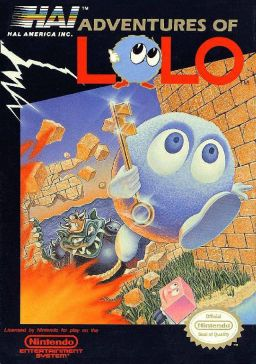
\includegraphics[width=0.3\linewidth]{./Figures/image_1.png}
  \end{center}
  \caption{Capa do jogo no NES}
  \label{fig:01}
\end{figure}

\section{Metodologia}
\label{sec:Metodologia}

Para implementação do jogo no RARS, utilizaram-se principalmente as ferramentas
\textit{bitmap display}, o que permite imprimir as imagens (sprites) dos personagens,
blocos, inimigos entre outros, criando uma interface visual para o jogador, e o
KDMMIOS (Keyboard and Display MMIO Simulator), o qual possibilita enviar um dado
do teclado para o RARS, viabilizando a movimentação do Lolo por meio do teclado
do jogador.

De início, o projeto começou com a criação de um repositório no GitHub para fins
de organização do grupo e melhor versionamento de código, assim, partimos para
implementação da impressão de sprites no bitmap display. Para tal, precisamos
formular uma estratégia para renderização dos sprites.

\subsection{Blocos 16x16}{
\label{sec:MIPS}

Percebemos no jogo original que os espaços por onde
o jogador e inimigos se movimentavam, como o espaço
em que os mesmos ocupavam, podia ser interpretado
como um bloco com 16 pixels de largura por 16 pixels de altura, assim implementamos o jogo assumindo
que cada elemento possuía como base um bloco 16x16
pixels.

}

\begin{figure}[htb]
  \begin{center}
   
\includegraphics[width=0.7\linewidth]{./Figures/image_2e3e4.png}
  \end{center}
  \caption{Sprites de 16x16 pixels}
  \label{fig:02}
\end{figure}

\begin{figure}[htb]
  \begin{center}
   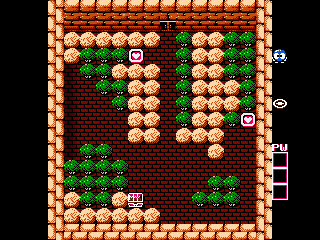
\includegraphics[width=0.3\linewidth]{./Figures/image_5.png}
  \end{center}
  \label{fig:01}
\end{figure}

Isso nos permitiu tratar as posições das imagens no bitmap display de forma mais
automática e fácil de visualizar e modificar, assim criamos os mapas de tal
forma que os blocos assumiam posições que eram divisíveis por 16, assim fizemos
mapa feitos com blocos 16x16. Devido a essa estratégia, o mapa de jogo não ocupa
completamente o bitmap display, sendo possível jogar em parte limitada apenas.
Por questões de estética, o mapa implementado é maior que o mapa do jogo
original, possuindo mais uma linha e colunas de blocos 16x16, caracterizando o
mapa jogável (paredes, chão, árvores) com 210 blocos 16x16, e o Bitmap Display
inteiro por 300 blocos 16x16.

\begin{figure}[htb]
  \begin{center}
   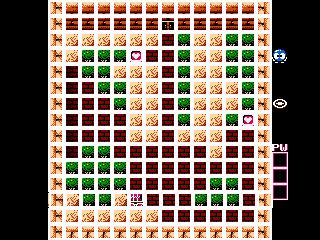
\includegraphics[width=0.3\linewidth]{./Figures/image_6.png}
  \end{center}
  \caption{ mapa criado por nós e visualização dos
blocos 16x16 no mapa jogável respecttivamente}
  \label{fig:01}
\end{figure}


\subsection{Colisão e matriz do mapa}{
\label{sec:Mars}
Como estratégia de colisão, decidimos fazer uso de
uma matriz para representar o Bitmap display, como
a tabela quadriculada na parte direita da figura 3.

}

\begin{figure}[htb]
  \begin{center}
   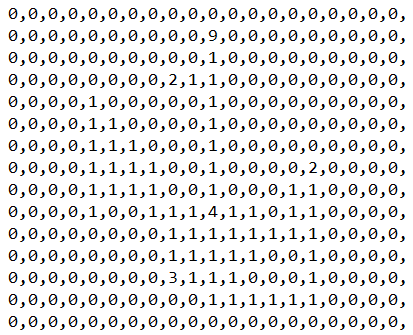
\includegraphics[width=0.3\linewidth]{./Figures/image_7.png}
  \end{center}
  \caption{ mapa criado por nós e visualização dos
blocos 16x16 no mapa jogável respecttivamente}
  \label{fig:01}
\end{figure}

Como o bitmap display possui 300 blocos 16x16, a matriz possui, também, 300
posições, com cada número representando o que o Lolo pode ou não fazer em cada
posição do mapa. Assim, enquanto movemos o Lolo pelo mapa, sua posição na matriz
também se modifica, sendo possível checar as posições, inimigos, paredes,
prêmios, entre outros. Colocamos a matriz como um array no RARS, sendo possível
sua interação. Para checar se o Lolo podia se mover entre os blocos, checava-se
as extremidades do quadrado em que o Lolo ocupava com as extremidades dos outros
blocos.


\begin{itemize}
    \item 0 - Lolo não pode se mover para além desse bloco
    \item 1 - Lolo pode se movimentar por entre esses blocos livremente
    \item 2 - Coração
    \item 3 - Baú
    \item 9 - Porta
\end{itemize}

Com isso, é possível checar as posições dos elementos estáticos (paredes e chão)
do mapa de forma rápida e fácil, porém, elementos dinâmicos, como o Lolo e os
inimigos que se movem, possuem a característica de nem sempre terem uma posição
estática ou podem se modificar quando o Lolo agir sobre algum bloco ou sprite.
Portanto, tivemos que implementar algo parecido com uma struct, junto com
alocamento de memória, como pode ser feita em linguagens de programação de mais
alto nível, como C.

\subsection{Blocos dinâmicos}{
\label{sec:MIPS}
O Lolo é o principal elemento dinâmico que ocupa um
bloco 16x16, já que ele se move em qualquer direção
que o jogador desejar e interage com os outros blocos
e inimigos, além do Lolo conseguir modificar alguma
parte do mapa.

}

\begin{figure}[htb]
  \begin{center}
   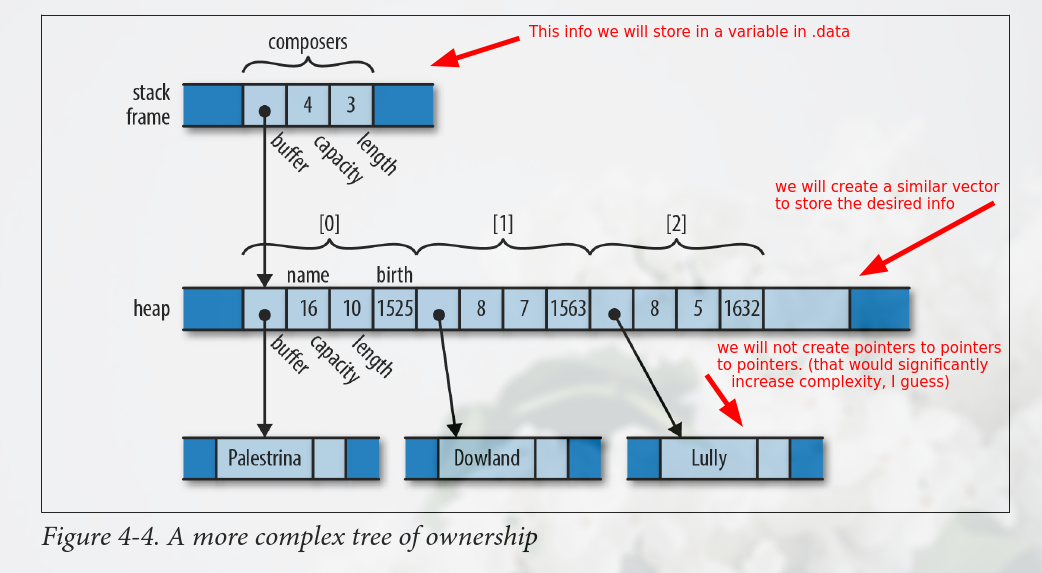
\includegraphics[width=0.3\linewidth]{./Figures/image_8.png}
  \end{center}
  \caption{Exemplificação de um array de structs
em Assembly. Imagem original de “Programming
Rust by Jim Blandy and Jason Orendorf}
  \label{fig:01}
\end{figure}

A partir dessa implementação, os blocos dinâmicos podiam ser tratados no RARS
com maior flexibilidade, o que possibilitou a movimentação do Lolo pelo mapa, de
forma que as impressões, dos movimentos do Lolo, passados pudessem ser pagadas
sem modificar o bloco por onde o Lolo se movimenta, como o bloco do chão de
tijolo.


\section{Resultados obtidos}
\label{sec:Resultados}

\subsection{Desafios}{
\label{sec:MIPS}
De início, encontramos um problema na colisão do
Lolo, em que dependendo do dado do teclado, em que
o jogador tentasse se mover diagonalmente, ele podia
passar por cima das paredes. Resolvemos ao checar
as extremidades do bloco em que o Lolo ocupava com
as extremidades do bloco por onde o jogador queria
que o Lolo se movimentasse, impedindo a impressão
ou não.

Outro problema foi a movimentação do Lolo de tal forma que suas imagens de
movimentações antigas fossem apagadas e que o bloco de tijolo fosse restaurado.
Resolvemos isso criando uma checagem nas struct, salvando o bloco original por
onde o Lolo se moveu }

\begin{figure}[htb]
  \begin{center}
   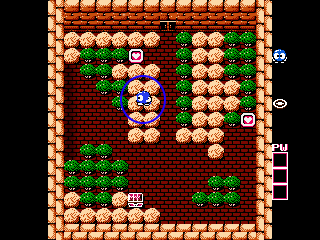
\includegraphics[width=0.3\linewidth]{./Figures/image_9.png}
  \end{center}
  \caption{}
  \label{fig:01}
\end{figure}

\begin{figure}[htb]
  \begin{center}
   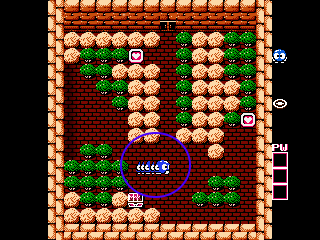
\includegraphics[width=0.3\linewidth]{./Figures/image_10.png}
  \end{center}
  \caption{Figura 7: colisão defeituosa e impressão
de animação defeituosa respectivamente.}
  \label{fig:01}
\end{figure}

Ao final conseguimos implementar muito bem a movimentação do Lolo junto com
animação e a colisão com paredes e outros elementos do mapa

\section{Conclusão}
Um grande benefício do projeto foi a criação de um ambiente de trabalho com o
grupo, demandando atenção, paciência, tempo e organização, o qual pode ser
proveitoso para situações futuras do mercado de trabalho ou em outros projetos
estudantis.

O Jogo em si teve alguns elementos que gostaríamos de ter implementado, mas
foram deixados de fora devido à uma certa falta de organização do tempo para
poder criá-los, já que a linguagem Assembly, apesar de ser simples, demanda uma
boa quantidade de tempo para poder utiliza-la eficientemente. Entretanto, foi
uma ótima oportunidade para a interação do grupo e para nossa própria formação
acadêmica e profissional, e conseguimos acumular uma ótima experiência que
servirá de referência no futuro


\section{Referência}
\label{sec:Conclusao}
\begin{itemize}
    \item[--] Aulas gravadas do professor Marcus Vinícius Lamar;
    \item[--] Aulas gravada de Thales Menezes;
    \item[--] The adventures of Lolo, \textit{\url{https://en.wikipedia.org/wiki/Adventures_of_Lolo}}.
    \item[--] Acesso em 17/05/2021.
    
\end{itemize}


%{\bf Acknowledgments}
%[Blind Review]

%\newcommand{\BIBdecl}{\setlength{\itemsep}{-0.5 em}}
%\bibliographystyle{IEEEtran}
\bibliographystyle{sbgames}
\bibliography{bibliography}

\end{document}
